\documentclass[journal,twoside,web]{IEEEtran}
% Manuscript v2 for IEEE Journal of Biomedical and Health Informatics (JBHI), 2026-10-20.
% Numbers: experiments/b1_cost_acquisition (frozen protocol PROTOCOL_B1.md, SHA-256 ad1acf74...),
% experiments/h1_stage_recheck, experiments/rna_transport; costs: cost_vector.json.
% Architecture figure restyled from Multimodal_Blockchain_Sustainability_Architecture.drawio.
% Blockchain components are specified as interfaces and are NOT evaluated; all such text is highlighted.
% Set \chainhlfalse below to remove the highlighting for the submission version.
\usepackage{cite}
\usepackage{amsmath,amssymb}
\usepackage{graphicx}
\usepackage{booktabs}
\usepackage{multirow}
\usepackage{array}
\usepackage[table]{xcolor}
\usepackage{soul}
\usepackage[most]{tcolorbox}
\usepackage[hidelinks]{hyperref}

\definecolor{chainfg}{HTML}{8A5A00}
\definecolor{chainbg}{HTML}{FDF0D2}
\newif\ifchainhl \chainhltrue
% \chainhlfalse   % <- uncomment to remove the blockchain highlighting (submission version)
\ifchainhl
  \sethlcolor{chainbg}
  \newcommand{\bc}[1]{\hl{#1}}
  \newcommand{\bct}[1]{\texorpdfstring{\colorbox{chainbg}{#1}}{#1}}
  \newtcolorbox{chainbox}[1][]{enhanced,breakable,colback=chainbg,colframe=chainfg,boxrule=0.5pt,
    arc=1.5pt,left=4pt,right=4pt,top=3pt,bottom=3pt,fonttitle=\bfseries\footnotesize,
    coltitle=chainfg,colbacktitle=chainbg,title={#1}}
\else
  \newcommand{\bc}[1]{#1}
  \newcommand{\bct}[1]{#1}
  \newtcolorbox{chainbox}[1][]{enhanced,breakable,colback=white,colframe=white,boxrule=0pt,
    left=0pt,right=0pt,top=0pt,bottom=0pt,fonttitle=\bfseries\footnotesize,coltitle=black,colbacktitle=white,title={#1}}
\fi
\newcommand{\todo}[1]{\textcolor{red}{[TODO: #1]}}
\graphicspath{{figures/}}

\begin{document}

\title{Stage Before Sequencing: Cost-Aware Sequential Modality Acquisition for Multimodal Survival Prediction in Non-Small Cell Lung Cancer}

\author{\todo{Author list and affiliations}%
\thanks{This work used only public, de-identified data (GDC/TCGA, CPTAC, GEO) \todo{confirm institutional data-use statement}.}%
\thanks{\ifchainhl\bc{Highlighted text} marks blockchain components of the proposed architecture. They are specified as software interfaces and were not deployed or evaluated in this study.\fi}}

\maketitle

\begin{abstract}
Multimodal models that fuse clinical variables, whole-slide images (WSIs) and transcriptomics are increasingly reported to outperform clinical baselines for cancer survival prediction, yet they implicitly assume that every modality is acquired for every patient. For sustainable health systems, the relevant question is which patients, if any, need each additional test, at what cost, and how such decisions can be traced. We formulate postoperative prognostication as cost-aware sequential acquisition along a clinicopathologic $\rightarrow$ H\&E WSI $\rightarrow$ RNA sequencing ladder and compare per-patient value-of-information (VoI) policies with random and static policies over 66 budget pairs, priced with literature-derived costs (WSI US\$12--78 and RNA sequencing US\$300--2,919 per patient). The analysis is embedded in an architecture that keeps evidence off-chain and \bc{reserves a smart-contract layer for anchoring each conclusion with its evidence hash}. In 1,313 patients with non-small cell lung cancer from TCGA and CPTAC, analyzed under a frozen protocol, a clinicopathologic model including pathologic stage reached a 3-year IPCW C-index of 0.644, against 0.645 for full WSI\,+\,RNA acquisition ($\Delta$\,=\,+0.001, 95\% CI $-$0.024 to +0.029); no costlier policy improved on the zero-cost policy beyond bootstrap uncertainty, and VoI selection did not outperform random selection after multiplicity correction. Without stage, WSI was the most cost-effective addition (0.580 $\rightarrow$ 0.610) and RNA sequencing helped only after universal WSI (0.622). The transcriptomic gain attenuated similarly in seven external cohorts (n\,=\,1,690; +0.073 to +0.022). Multimodal prognostic models should be compared against baselines that contain all information available at the prediction time and reported with explicit acquisition costs.
\end{abstract}

\begin{IEEEkeywords}
Multimodal learning, survival analysis, cost-sensitive learning, value of information, sustainable healthcare, computational pathology, non-small cell lung cancer, \bc{blockchain}.
\end{IEEEkeywords}

%====================================================================
\section{Introduction}
\IEEEPARstart{M}{ultimodal} deep learning that combines routine clinical variables with histopathology and molecular profiles has become a standard recipe for cancer prognostication~\cite{cheerla2019,chen2022,valesilva2021}. Reported gains over clinical baselines motivate a picture in which every patient receives digitized slides and a transcriptome. That picture is expensive. Whole-transcriptome sequencing costs hundreds to thousands of US dollars per patient and takes up to two working weeks~\cite{altburger2026,ortendahl2025,cuppen2022}. Digital pathology adds scanner, staff and storage costs~\cite{ardon2023} and a carbon footprint dominated by image storage~\cite{tilmant2026,vafaeisadr2024}. Whether a modality is worth acquiring is therefore not answered by its average discrimination gain alone. The question is for whom it changes the prognosis enough to justify its cost.

Sustainability in health care has several layers: money, time, laboratory capacity, equitable access in resource-limited settings, and environmental impact. A prognostic model that silently requires sequencing for every patient is unsustainable on all of them. Recent work has started to treat modality acquisition as a sequential decision. SAGEAgent, for example, acquires modalities per patient while trading survival performance against acquisition burden~\cite{qu2026}, building on general dynamic feature selection~\cite{covert2023,ji2007,shim2018}. Large benchmarks have also standardized multi-omics survival evaluation~\cite{wissel2025}. What has received less attention is how strongly such conclusions depend on what the clinical baseline already knows at the prediction time, and on how discrimination is computed.

Two issues make the average gain itself fragile. First, the clinical baseline often omits pathologic stage, although stage is available after resection, which is exactly when the surgical specimen used for WSI and RNA becomes available. Imaging and molecular features partly encode stage, so an apparent modality gain can partly reflect stage information. Second, implementations of the inverse-probability-of-censoring-weighted (IPCW) C-index~\cite{uno2011} differ in how they treat patients followed beyond the truncation time, which can change the estimated gain~\cite{sonabend2022}.

A third issue concerns accountability. When a model's output is used to withhold or allocate a test, the decision, the model version and the evidence behind it should be traceable later, possibly by parties who do not trust each other. \bc{Distributed ledgers have been proposed for exactly this kind of multi-party audit in health data}~\cite{kuo2017,azaria2016}. We therefore place the acquisition analysis inside an architecture (Fig.~\ref{fig:arch}) that stores evidence off-chain and \bc{reserves an on-chain layer for compact, verifiable records of each conclusion}. This paper evaluates the analysis layers; \bc{the blockchain layers are specified as interfaces for later evaluation}.

Our contributions are:
\begin{enumerate}
\item A per-patient acquisition formulation along a clinicopathologic $\rightarrow$ WSI $\rightarrow$ RNA ladder, evaluated with VoI, random and static policies over a two-dimensional budget grid, under a protocol frozen before any policy was run.
\item A literature-sourced cost vector (money, turnaround, carbon) for WSI and RNA sequencing, with explicit derivations and a statement of what could not be quantified.
\item Evidence, internal and external, that with a stage-inclusive baseline neither WSI nor RNA sequencing adds detectable discrimination in this cohort, and that without stage the cost-performance frontier is ordered ``WSI first, RNA second''.
\item A quantification of how one IPCW C-index implementation choice, which we had used in an earlier stage of this project, inflated the fusion gain.
\item \bc{A governance architecture and a backend-agnostic ledger interface that anchors each analysis conclusion with the hash of its evidence, with a working local reference implementation and a reserved blockchain backend.}
\end{enumerate}

\begin{figure*}[t]
\centering
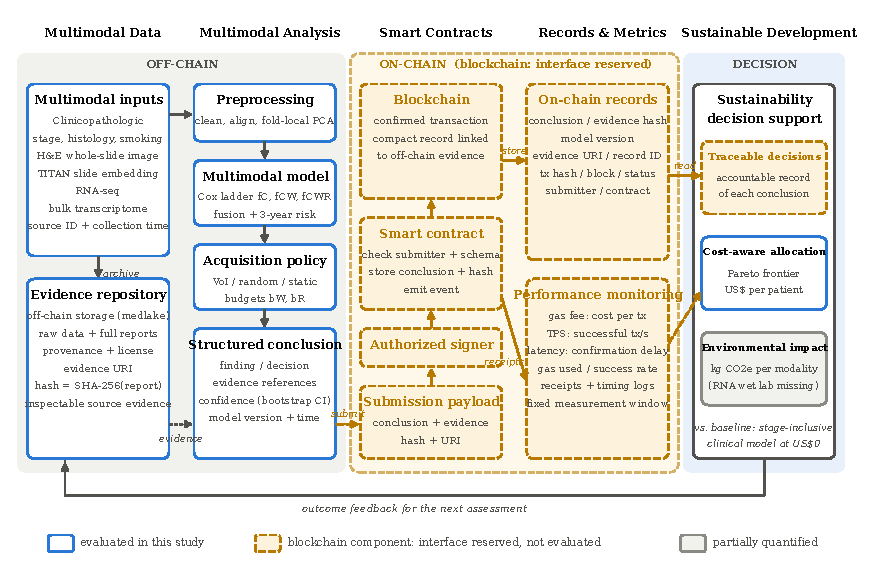
\includegraphics[width=\textwidth]{fig0_architecture.pdf}
\caption{System architecture, restyled from the authors' architecture diagram. Off-chain layers (left) hold multimodal inputs, an evidence repository with SHA-256 hashes, and the multimodal analysis that produces a structured conclusion. \bc{The on-chain layers (amber, dashed) would anchor a compact payload (conclusion, evidence hash, URI) through a smart contract, store on-chain records and monitor gas, throughput and latency.} The decision layer turns records into sustainability decisions; the cost-aware allocation (blue) is the part evaluated in this study, while environmental impact is only partially quantified. Outcomes feed back into the next assessment.}
\label{fig:arch}
\end{figure*}

%====================================================================
\section{Related Work}
\subsection{Multimodal Survival Prediction and Benchmarks}
Fusion of histology and genomics improved pan-cancer prognostication over single modalities in several studies~\cite{chen2022,cheerla2019,valesilva2021}. SurvBoard standardized multi-omics survival benchmarking across 28 cancer datasets, including clinical comparators and missing modalities~\cite{wissel2025}. The MMIST-LUNG release, which we use, curated TCGA and CPTAC lung cancer cases with clinical, WSI, transcriptomic, CT and PET data and non-uniform missingness~\cite{mendes_mmist}. These works mostly assume complete acquisition at test time. Our results suggest that the information content of the clinical baseline at the chosen prediction time is decisive for the size of the multimodal gain.

\subsection{Cost-Aware and Dynamic Feature Acquisition}
Acquiring features sequentially under a budget is well studied in machine learning~\cite{ji2007,shim2018,covert2023}. Most methods target classification and estimate the value of the next feature by its expected information gain or loss reduction. SAGEAgent applies agent-based acquisition to multimodal survival prediction and uses the probability of a risk change as an acquisition signal~\cite{qu2026}. We use a deliberately simple VoI proxy, the predicted change in 3-year risk, and ask whether it beats random selection when the baseline is strong; Section~\ref{sec:voi-theory} states when such a proxy is justified.

\subsection{Evaluation of Survival Discrimination}
Uno's IPCW C-index~\cite{uno2011} is the standard truncated concordance measure; implementation choices and transformations of risk predictions can change C-index values substantially~\cite{sonabend2022}. We report a specific instance from our own pipeline rather than a claim about the literature.

\subsection{Sustainability of Digital Pathology and Genomics}
Recent analyses quantify the operational cost of clinical-scale digital pathology~\cite{ardon2023}, its greenhouse-gas emissions~\cite{tilmant2026,vafaeisadr2024}, the micro-costs of clinical sequencing~\cite{altburger2026,cuppen2022,kumar2022}, and the carbon footprint of bioinformatic analysis~\cite{grealey2022}. We connect these figures to the predictive value of the modalities they price.

\subsection{\bct{Blockchain for Health Data Governance}}
\begin{chainbox}[Blockchain component]
Distributed ledgers have been proposed for consent management, access control and audit trails in biomedical research and health care~\cite{kuo2017,azaria2016}. Permissioned platforms such as Hyperledger Fabric allow several organizations to endorse transactions without a single administrator~\cite{androulaki2018}. A recurring criticism is that many proposals would work equally well with a signed centralized log. We therefore specify the ledger as an interface with a centralized hash-chained log as its reference backend, so that a later evaluation can compare the two directly.
\end{chainbox}

%====================================================================
\section{System Architecture}
\label{sec:arch}
Fig.~\ref{fig:arch} shows the five layers. Each is described with the component that implements it in our code.

\textit{Multimodal data.} Inputs are clinicopathologic variables, H\&E WSIs and bulk RNA. Each record carries its source identifier and collection time. Files are stored in a local data lake that records provenance, license and a SHA-256 checksum for each file; this is the off-chain evidence repository.

\textit{Multimodal analysis.} Fold-local preprocessing, a ladder of Cox models and an acquisition policy (Section~\ref{sec:methods}) produce a structured conclusion: the finding or decision, references to the evidence files, a confidence statement (bootstrap interval) and the model version with a timestamp. The evidence hash is $H(\text{sorted list of evidence paths and their SHA-256})$.

\begin{chainbox}[Blockchain layers: smart contracts, on-chain records, performance monitoring]
\textit{Smart-contract anchoring.} A submission payload contains the conclusion, the evidence hash and the evidence URI. An authorized signer submits it; the contract checks the submitter and the record schema, stores the conclusion and evidence hash, and emits an event. Only compact records go on-chain; full evidence stays off-chain and can be re-hashed by an auditor.

\textit{On-chain records.} Stored fields are the conclusion, evidence hash, model version, evidence URI and record ID, plus transaction metadata (transaction hash, block number, status, submitter and contract address).

\textit{Performance monitoring.} Gas per transaction, throughput (successful transactions per second) and confirmation latency are computed off-chain from receipts and timing logs over a fixed measurement window.
\end{chainbox}

\textit{Sustainable development.} Decision support combines cost-aware allocation (evaluated here as a cost-performance frontier in US dollars), environmental impact per modality (partially quantified) and \bc{traceable decisions (which depend on the on-chain layer)}. Each assessment is compared with a baseline, here the stage-inclusive clinical model at zero incremental cost, and outcomes feed back into the next assessment.

\begin{table}[t]
\centering
\caption{\bct{Ledger Interface: Event Used by the Analysis Layer}}
\label{tab:iface}
\setlength{\tabcolsep}{3pt}
\rowcolors{2}{chainbg}{chainbg}
\begin{tabular}{@{}>{\raggedright}p{2.0cm}>{\raggedright\arraybackslash}p{6.1cm}@{}}
\toprule
Item & Specification \\
\midrule
Event & \texttt{ANALYSIS\_RECORD} \\
Payload & record\_id, conclusion ($\le$512 characters), evidence\_hash, evidence\_uri, model\_version, confidence \\
Rejected fields & patient key or ID, salts, feature values \\
Contract checks & authorized submitter; complete schema \\
Receipt & tx hash, block number, previous hash, status, submitter, contract, submit and confirm times, gas used \\
Backends & local hash-chained log (implemented); permissioned blockchain (interface reserved, not evaluated) \\
\bottomrule
\end{tabular}
\end{table}

%====================================================================
\section{Problem Formulation}
\label{sec:problem}
\subsection{Prediction Task and Estimand}
For patient $i$ let $T_i$ be overall survival time from the GDC index date, $C_i$ the censoring time, and $\tau = 1095$ days. Modalities are acquired in a fixed order $m \in \{0,1,2\}$: clinicopathologic data including pathologic stage ($X^{(0)}$), plus WSI ($X^{(1)}$), plus RNA ($X^{(2)}$). Because WSI and RNA come from resection specimens and pathologic stage is available after surgery, the prediction time point is postoperative. The model at level $m$ outputs a 3-year event probability $r^{(m)}_i = 1 - \hat S_m(\tau \mid X^{(0)}_i,\dots,X^{(m)}_i)$, so that patients scored at different levels can be ranked on one scale. The estimand is the 3-year Uno C-index of the resulting risk vector in the target population, together with the expected incremental acquisition cost per patient.

\subsection{Acquisition Policies}
A policy is defined by budgets $b_W, b_R \in \{0, 0.1, \dots, 1\}$ with $b_R \le b_W$ (66 pairs) and two scores $s_W, s_R$. The top-$b_W$ fraction of patients by $s_W$ receives WSI; among them, the top fraction $b_R$ of all patients by $s_R$ receives RNA. Each patient keeps the risk of the highest level acquired:
\begin{equation}
r_i = \begin{cases} r^{(2)}_i & i \in \mathcal{R},\\ r^{(1)}_i & i \in \mathcal{W}\setminus\mathcal{R},\\ r^{(0)}_i & \text{otherwise,}\end{cases}
\end{equation}
with expected cost per patient $c(b_W, b_R) = b_W c_W + b_R c_R$.

\subsection{Why Predicted Risk Change Is a Reasonable VoI Proxy}
\label{sec:voi-theory}
Let $Y = \mathbb{1}\{T \le \tau\}$ (ignoring censoring for this argument), $p_0 = P(Y{=}1 \mid X^{(0)})$ and $p_1 = P(Y{=}1 \mid X^{(0)}, X^{(1)})$. Since $(Y-p_0)^2-(Y-p_1)^2 = (p_1-p_0)(2Y-p_0-p_1)$ and $E[Y \mid X^{(0)},X^{(1)}] = p_1$,
\begin{equation}
E\big[(Y-p_0)^2-(Y-p_1)^2 \,\big|\, X^{(0)}\big] = E\big[(p_1-p_0)^2 \,\big|\, X^{(0)}\big].
\end{equation}
The expected reduction in Brier loss~\cite{brier1950} from acquiring $X^{(1)}$ therefore equals the expected squared change in risk when both models are calibrated conditional probabilities. Ranking patients by predicted $|r^{(1)} - r^{(0)}|$ is thus a principled proxy, and its failure in practice points to miscalibration, finite-sample error or model disagreement rather than to a wrong objective. The identity concerns a decomposable loss; a C-index gain is not a sum of per-patient gains.

%====================================================================
\section{Materials and Methods}
\label{sec:methods}
Reporting follows TRIPOD~\cite{collins2015} where applicable.

\subsection{Cohort}
We used the MMIST-LUNG curation~\cite{mendes_mmist} of TCGA-LUAD, TCGA-LUSC, CPTAC-LUAD and CPTAC-LSCC~\cite{tcga_luad,tcga_lusc,gillette2020,satpathy2021}. Overall survival was reconstructed from GDC case records using explicit vital status and positive follow-up or death times; deaths without a valid time were never treated as censored. Of 1,365 patients, 52 were excluded (39 with unknown status or death without a valid time, 11 alive without positive follow-up, 2 without a local GDC record). Table~\ref{tab:cohort} summarizes the 1,313 analyzed patients. Pathologic stage groups were reconstructed from the raw GDC diagnoses with the same rules used for the external cohorts; 12 missing values were kept as a separate category.

\begin{table}[t]
\centering
\caption{Analysis Cohort}
\label{tab:cohort}
\setlength{\tabcolsep}{4pt}
\begin{tabular}{@{}lrrrr@{}}
\toprule
 & TCGA & CPTAC & Total \\
\midrule
Patients & 1,005 & 308 & 1,313 \\
\quad LUAD / squamous & 509 / 496 & 206 / 102 & 715 / 598 \\
Deaths & 397 & 87 & 484 \\
With WSI features & 1,005 & 305 & 1,310 \\
With RNA features & 997 & 308 & 1,305 \\
\midrule
\multicolumn{4}{@{}l}{Pathologic stage: I 666, II 371, III 230, IV 34, missing 12} \\
\multicolumn{4}{@{}l}{Median observed time: 669 days} \\
\bottomrule
\end{tabular}
\end{table}

\subsection{Modalities and Features}
\textit{Clinicopathologic (level 0):} ten-year age bin, sex, race, ethnicity, smoking status, pack-years and smoking years, ICD-10 code, morphology, prior malignancy, and pathologic stage group (I--IV). A contrast analysis removes stage. \textit{WSI (level 1):} author-provided 768-dimensional TITAN slide embeddings~\cite{titan}, averaged per patient (4,532 slides). \textit{RNA (level 2):} author-provided bulk transcriptome features (10,270 features). Within each training fold, the WSI and RNA blocks were reduced by keeping the 256 highest-variance features, standardizing and projecting onto 16 principal components. CT and PET features were available for only 68 and 30 patients and were not used.

\subsection{Prognostic Models}
Within each of five outer folds (stratified by source and event; seed 20261004), we fitted three Breslow Cox models with a ridge penalty $\alpha \in \{1, 10, 100\}$ selected by Harrell's C on an inner 20\% validation split~\cite{polsterl2020}: $f_C$ (clinicopathologic), $f_{CW}$ (adding the WSI block and a presence indicator) and $f_{CWR}$ (adding the RNA block and indicator). Patients lacking a modality (3 for WSI, 8 for RNA) were handled through the presence indicators. Each test fold held about 263 patients.

\subsection{Acquisition Policies}
\textit{VoI policy.} Training targets were the absolute risk changes $d_W = |r_{CW} - r_C|$ and $d_R = |r_{CWR} - r_{CW}|$, obtained on the outer training set by inner five-fold cross-fitting, with all three Cox models refitted in each inner fold. Gradient-boosted regressors (depth 3, learning rate 0.05, 200 iterations) predicted $d_W$ from level-0 features and $d_R$ from level-0 plus WSI features. \textit{Random policy:} the same budgets, averaged over 100 random selections per fold. \textit{Static policies:} the corners of the grid. \textit{Risk-change oracle:} ranks test patients by their true $d$, i.e.\ by how much the fuller model would move their risk. It is a diagnostic reference for the VoI regressor, not an upper bound on attainable discrimination, because a large risk change need not improve the ranking.

\subsection{Cost Vector}
Costs are incremental to standard care (Table~\ref{tab:cost}). For WSI we summed scanner ownership (US\$0.55--19.53 per slide), scanning staff (US\$0.79--0.92) and on-premise storage (2\,GB per slide at US\$1\,M per petabyte including redundancy, i.e.\ US\$2.00) from a clinical-scale operation~\cite{ardon2023}, and multiplied by the observed 3.46 slides per patient. For RNA sequencing we used a lower bound of WTS consumables (\texteuro278 per case~\cite{altburger2026}; US\$300 at an assumed 1.08\,US\$/\texteuro) and an upper bound of a clinical whole-exome/whole-transcriptome test (US\$2,919~\cite{ortendahl2025}). Two scenarios span the plausible cost ratio: \emph{low ratio} (WSI \$78, RNA \$300; $\kappa = 3.9$) and \emph{high ratio} (WSI \$12, RNA \$2,919; $\kappa = 253$). Because policies are defined by acquisition fractions, any other cost vector maps onto the same results without refitting. These are scenario values from the literature, not measured costs in our setting; if RNA or scanning is already performed for another clinical purpose, its incremental prognostic cost is zero.

\begin{table}[t]
\centering
\caption{Incremental Acquisition Cost Vector per Patient}
\label{tab:cost}
\setlength{\tabcolsep}{3pt}
\begin{tabular}{@{}p{1.5cm}p{3.1cm}p{3.15cm}@{}}
\toprule
 & H\&E WSI & RNA sequencing \\
\midrule
Monetary (US\$) & 11.6--77.7 (3.34--22.45 per slide $\times$ 3.46 slides)~\cite{ardon2023} & 300 (consumables only)~\cite{altburger2026} to 2,919 (clinical WES/WTS)~\cite{ortendahl2025} \\
Turnaround & $\approx$1 min scanning per slide (modelling assumption); same day~\cite{vafaeisadr2024} & $<$10--14 working days (WGTS)~\cite{cuppen2022} \\
Carbon (kg CO$_2$e) & 0.25--0.35 (0.073--0.101 per slide incl.\ 1-year storage; French grid)~\cite{tilmant2026} & $\ge$0.05--5 (alignment compute only, 50\,M reads)~\cite{grealey2022}; wet lab not quantified \\
\bottomrule
\end{tabular}
\end{table}

\subsection{Evaluation and Statistics}
The primary metric was the 3-year Uno IPCW C-index~\cite{uno2011}, with the censoring distribution estimated on the outer training set and patients with $t \ge \tau$ retained as comparators, averaged over folds. Our matrix implementation matched scikit-survival to within $10^{-10}$, including on bootstrap resamples. Secondary metrics were the 3-year cumulative/dynamic AUC and IPCW Brier score. Uncertainty used a paired bootstrap of test patients within folds (2,000 replicates, seed 20261008; 500 for off-diagonal grid points); all policies shared the same resamples, and fold-wise differences were averaged before taking percentiles. Intervals condition on the fitted models.

Four questions were prespecified. Q1 asked for the smallest RNA budget $b_R^*$ (with WSI for all) whose difference from RNA-for-all had a 95\% lower bound above $-\delta$, with $\delta = 0.01$. Q2 compared VoI with random selection at $b_R \in \{0.1, 0.2, 0.3, 0.5\}$ with Holm correction. Q3 computed cost-performance frontiers. Q4 repeated everything without stage. A depth-2 decision tree was prespecified to summarize which patients the VoI policy selects at $b_R^*$.

\subsection{External Transportability of the RNA Branch}
In a separately frozen analysis, a single RNA\,+\,clinical Cox model was trained on the development cohort (GDC STAR-Counts TPM, 10,902 genes shared with all platforms, within-sample rank normalization) and applied unchanged to seven GEO microarray cohorts~\cite{edgar2002} on four platforms (1,690 patients, 718 deaths). Cohort-level differences were pooled by DerSimonian--Laird random effects~\cite{dersimonian1986}.

\subsection{Reproducibility and \bct{Anchoring of Results}}
The protocol was frozen with a SHA-256 record before any policy was run, and the analysis script verifies that hash at run time; there were no deviations. The analysis ran on CPU only. \bc{As a reference for the governance layer, the frozen results were turned into two \texttt{ANALYSIS\_RECORD} payloads and appended to the local hash-chained log through the ledger interface; an auditor step recomputes the evidence hash from the files.}

%====================================================================
\section{Results}
\subsection{Static Policies}
With stage, the clinicopathologic model achieved a 3-year C-index of 0.644 (95\% CI 0.617--0.673), WSI for all 0.638 (0.610--0.667) and WSI\,+\,RNA for all 0.645 (0.618--0.674) (Fig.~\ref{fig:static}). Without stage the corresponding values were 0.580 (0.550--0.607), 0.610 (0.582--0.639) and 0.622 (0.596--0.650). WSI therefore contributed $+0.030$ and RNA a further $+0.012$ only when the baseline lacked stage.

\begin{figure}[t]
\centering
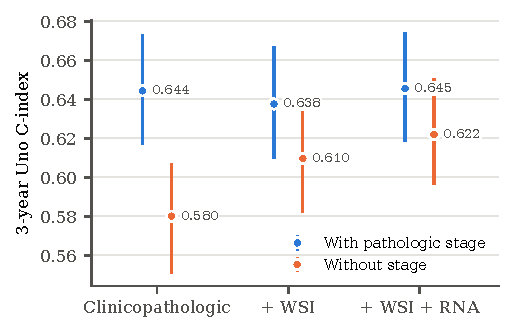
\includegraphics[width=\columnwidth]{fig2_static.pdf}
\caption{Static policies: 3-year Uno C-index (5-fold mean, 95\% bootstrap CI) for the three acquisition levels, with and without pathologic stage in the clinical baseline.}
\label{fig:static}
\end{figure}

\subsection{How Much RNA Sequencing Is Needed (Q1)}
Table~\ref{tab:q1} lists the differences from RNA-for-all. Across all budgets the point difference lay between $-0.008$ and $+0.001$ with stage and between $-0.012$ and $+0.001$ without (Fig.~\ref{fig:ni}). The prespecified rule returned $b_R^* = 0.8$ in both settings. This value reflects precision rather than benefit. At low budgets the 95\% interval half-width ($\approx$0.02 with about 263 test patients per fold) exceeds $\delta$, whereas intervals narrow mechanically as the policy converges to RNA-for-all. The prespecified decision tree, trained to reproduce the top-80\% selection, predicted ``acquire'' in every leaf in all folds and yielded no discriminating rule. The absence of a detectable difference is not evidence of equivalence; the intervals at low budgets cannot exclude losses of about 0.02.

\begin{table}[t]
\centering
\caption{Q1: Difference in 3-Year C-Index from RNA Sequencing for All (WSI for All)}
\label{tab:q1}
\setlength{\tabcolsep}{4pt}
\begin{tabular}{@{}lll@{}}
\toprule
$b_R$ & With stage & Without stage \\
\midrule
0.0 & $-0.008$ ($-0.026$, 0.010) & $-0.012$ ($-0.034$, 0.007) \\
0.1 & $+0.000$ ($-0.017$, 0.018) & $-0.006$ ($-0.026$, 0.013) \\
0.2 & $-0.006$ ($-0.023$, 0.011) & $+0.001$ ($-0.017$, 0.019) \\
0.3 & $-0.006$ ($-0.021$, 0.010) & $-0.004$ ($-0.021$, 0.013) \\
0.5 & $-0.007$ ($-0.019$, 0.005) & $-0.001$ ($-0.016$, 0.013) \\
0.7 & $-0.004$ ($-0.012$, 0.004) & $-0.001$ ($-0.011$, 0.009) \\
0.8 & $-0.002$ ($-0.008$, 0.004)$^{*}$ & $-0.001$ ($-0.008$, 0.007)$^{*}$ \\
0.9 & $+0.001$ ($-0.003$, 0.005) & $-0.002$ ($-0.007$, 0.003) \\
\bottomrule
\multicolumn{3}{@{}l}{\footnotesize $^{*}$Smallest budget meeting the prespecified criterion ($b_R^*$).}
\end{tabular}
\end{table}

\begin{figure*}[t]
\centering
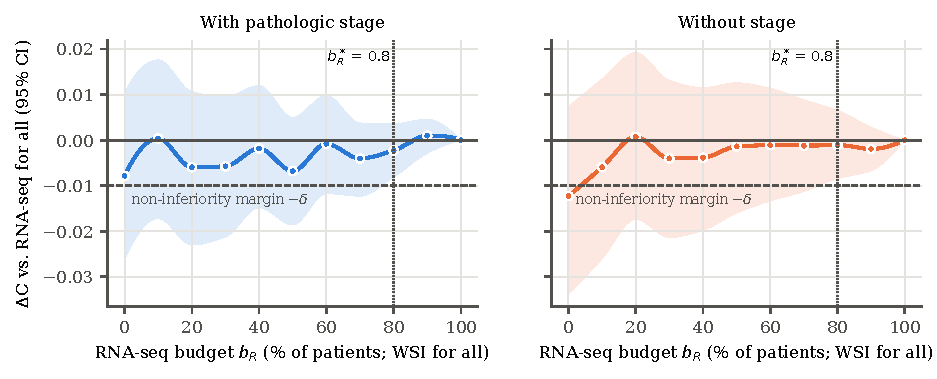
\includegraphics[width=0.85\textwidth]{fig3_noninferiority.pdf}
\caption{Q1. Difference in 3-year C-index between the VoI policy at RNA budget $b_R$ (WSI for all) and RNA sequencing for all, with 95\% paired-bootstrap CI. Dashed: margin $-\delta = -0.01$. Dotted: $b_R^*$. No budget shows a detectable loss; $b_R^*$ is driven by interval width. Markers are the evaluated budgets; curves and band are shape-preserving (PCHIP) interpolation between them.}
\label{fig:ni}
\end{figure*}

\subsection{VoI Versus Random Selection (Q2)}
The VoI regressors predicted the realized risk change only weakly: test-set Spearman $\rho$ was 0.18--0.36 for the RNA step and $-0.03$ to 0.25 for the WSI step across folds and settings. With stage, VoI exceeded random selection at $b_R = 0.1$ by $+0.008$ (95\% CI 0.001--0.015; raw $p = 0.021$, Holm $p = 0.084$) and was indistinguishable at 0.2, 0.3 and 0.5. Without stage, the largest difference was $+0.011$ at $b_R = 0.2$ (0.001--0.020; raw $p = 0.030$, Holm $p = 0.12$) (Fig.~\ref{fig:voi}). No comparison survived correction. The risk-change oracle exceeded random selection by at most about 0.016 C-index; because it ranks by risk change rather than by contribution to correct ordering, this does not bound what other selection rules could achieve.

\begin{figure*}[t]
\centering
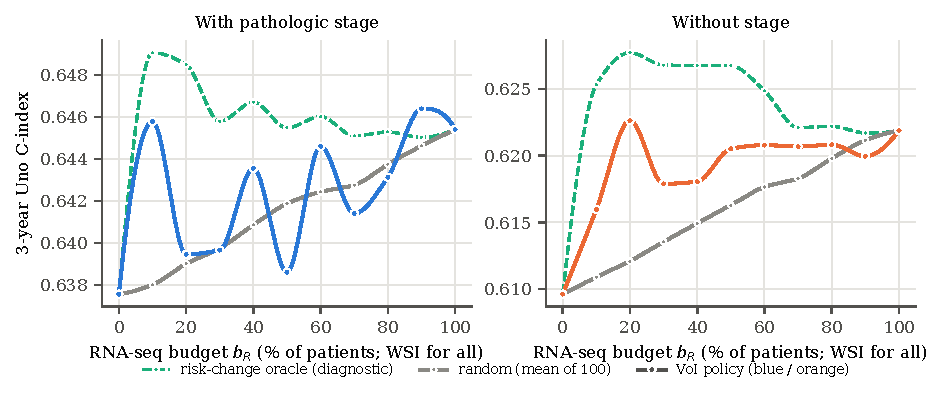
\includegraphics[width=0.85\textwidth]{fig5_voi_vs_random.pdf}
\caption{Q2. 3-year C-index of VoI, random (mean of 100 draws) and risk-change-oracle selection versus RNA budget, with WSI acquired for all patients. The oracle ranks patients by their true risk change and is a diagnostic reference, not an upper bound. Markers are the evaluated budgets; curves are shape-preserving (PCHIP) interpolation between them.}
\label{fig:voi}
\end{figure*}

\subsection{Cost-Performance Frontiers (Q3, Q4)}
The zero-cost policy is the cheapest point and therefore always on the frontier; the informative question is whether any costlier point improves on it. With stage, only two such points existed in both cost scenarios ($b_W = 0.5$ or $0.6$ with $b_R = 0.1$), with C-index 0.647 and 0.650, i.e.\ $+0.003$ and $+0.006$ above the zero-cost policy and well inside its interval (0.617--0.673) (Table~\ref{tab:pareto}, Fig.~\ref{fig:pareto}, top). Their expected cost was US\$69--77 per patient in the low-ratio and US\$298--299 in the high-ratio scenario. Without stage, the frontier rose along the WSI axis first, reaching 0.610 with WSI for all at US\$12--78 per patient, and admitted RNA only afterwards: 0.616 at $b_R = 0.1$ and 0.623 at $b_R = 0.2$, at US\$108--138 (low ratio) or US\$304--595 (high ratio) per patient (Fig.~\ref{fig:pareto}, bottom). Secondary metrics were flat across RNA budgets with stage (3-year AUC 0.682--0.692; Brier 0.208--0.211) and without stage (AUC 0.649--0.663; Brier 0.215--0.220).

\begin{table}[t]
\centering
\caption{Frontier Points Above the Zero-Cost Policy}
\label{tab:pareto}
\setlength{\tabcolsep}{3.5pt}
\begin{tabular}{@{}llrrl@{}}
\toprule
Baseline & ($b_W$, $b_R$) & \multicolumn{2}{c}{US\$/patient} & C-index (95\% CI) \\
 & & low & high & \\
\midrule
With stage & (0, 0) & 0 & 0 & 0.644 (0.617, 0.673) \\
 & (0.5, 0.1) & 69 & 298 & 0.647 (0.619, 0.675) \\
 & (0.6, 0.1) & 77 & 299 & 0.650 (0.624, 0.681) \\
\midrule
Without stage & (0, 0) & 0 & 0 & 0.580 (0.550, 0.607) \\
 & (1, 0) & 78 & 12 & 0.610 (0.582, 0.639) \\
 & (1, 0.1) & 108 & 304 & 0.616 (0.590, 0.646) \\
 & (1, 0.2) & 138 & 595 & 0.623 (0.597, 0.654) \\
\bottomrule
\multicolumn{5}{@{}p{8.4cm}@{}}{\footnotesize Without stage, intermediate WSI-only frontier points are omitted. Low/high: low and high RNA:WSI cost-ratio scenarios (Table~\ref{tab:cost}).}
\end{tabular}
\end{table}

\begin{figure*}[t]
\centering
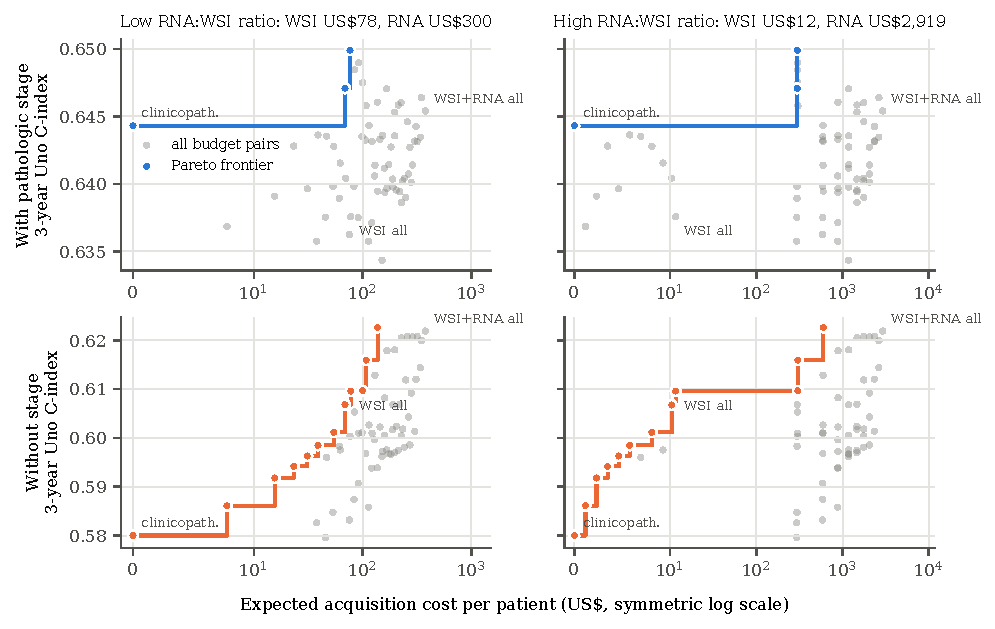
\includegraphics[width=0.92\textwidth]{fig4_pareto_usd.pdf}
\caption{Q3/Q4. Cost-performance frontiers in US dollars per patient for the 66 budget pairs (gray) under low and high RNA:WSI cost ratios (Table~\ref{tab:cost}). Top: baseline with pathologic stage; bottom: without stage. Points above the zero-cost policy in the top row lie within its bootstrap interval.}
\label{fig:pareto}
\end{figure*}

\subsection{Stage Attenuation Internally and Externally}
Against a stage-free clinical baseline, full WSI\,+\,RNA fusion gained $+0.042$ (95\% CI 0.008--0.077; $p = 0.012$) internally. With stage the gain was $+0.001$ ($-0.024$ to 0.029; $p = 0.96$), and with the full prespecified TNM coding $+0.004$ ($-0.019$ to 0.029). In the seven external GEO cohorts the RNA branch gained $+0.073$ (0.043--0.103; $I^2 = 0.25$) without and $+0.022$ ($-0.001$ to 0.045; $I^2 = 0.41$) with stage; six of seven cohort estimates were positive with stage (Fig.~\ref{fig:forest}). These results show that the measured increment depends strongly on the information in the baseline. They do not by themselves show that the image and molecular features contain nothing beyond stage, which would require stronger representations and models to test.

\begin{figure}[t]
\centering
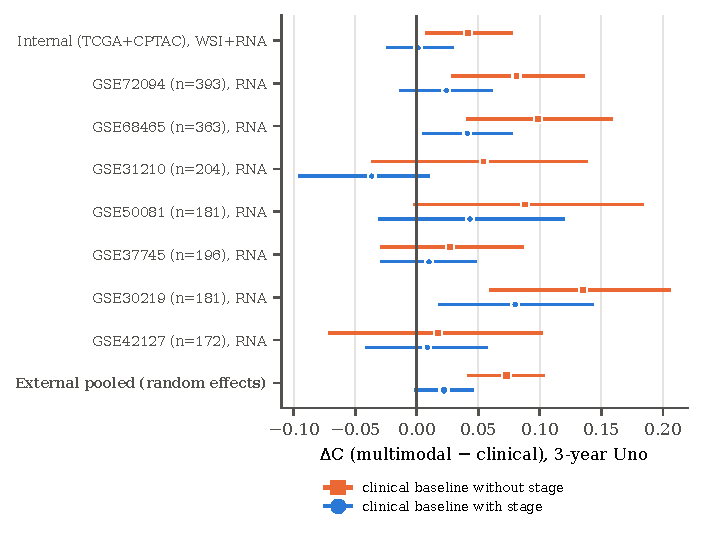
\includegraphics[width=\columnwidth]{fig6_stage_attenuation.pdf}
\caption{Attenuation of multimodal gains when pathologic stage enters the clinical baseline. Internal: WSI\,+\,RNA fusion in TCGA+CPTAC (5-fold). External: RNA\,+\,clinical model trained once on the development cohort and applied to seven GEO cohorts; pooled by random effects.}
\label{fig:forest}
\end{figure}

\subsection{Sensitivity to the IPCW Implementation}
An implementation we had used in an earlier stage of this project discarded test patients followed beyond $\tau$ before computing concordance, instead of retaining them as comparators as in Uno's estimator. It reported the internal stage-free fusion gain as $+0.071$ (0.031--0.108) instead of $+0.042$, an inflation of about 70\%, because the excluded long-term survivors are the most informative comparators for early events. With stage, the same implementation gave $+0.022$ ($-0.007$ to 0.051), leading to the same qualitative conclusion.

\subsection{\bct{Reference Implementation of the Governance Interface}}
\begin{chainbox}[Blockchain component: functional checks only]
Both frozen B1 conclusions (with and without stage) were appended as \texttt{ANALYSIS\_RECORD} events to the local hash-chained log. The chain verified and the recomputed evidence hash matched both records; in the interface test suite, payloads carrying patient identifiers were rejected by the schema check and an altered log entry was detected. These are functional checks of the interface on a single machine. They say nothing about the gas cost, throughput, latency or tamper resistance of a blockchain deployment, which remain to be measured with the reserved backend.
\end{chainbox}

%====================================================================
\section{Discussion}
\subsection{Principal Findings}
In postoperative NSCLC prognostication with a stage-inclusive baseline, neither digitized histology nor bulk transcriptomics added detectable discrimination in this cohort, and no costlier acquisition policy improved on the policy that uses only information routine pathology already produces. Per-patient VoI selection could not identify a subgroup for which RNA sequencing was worth its cost. Without stage, the picture changed: WSI then carried much of the missing information at a cost one to two orders of magnitude below RNA sequencing and entered the frontier first.

\subsection{Relation to Prior Work}
Our setting differs from SAGEAgent~\cite{qu2026} in disease, modalities and baseline, and we did not reproduce that method; the comparison we can make is conceptual. Both approaches use a risk-change signal to decide acquisition. Section~\ref{sec:voi-theory} shows when this signal equals the expected Brier gain; our weak Spearman correlations show that, with a strong baseline, it can be hard to predict from the information available before acquisition. Benchmarks such as SurvBoard~\cite{wissel2025} already include clinical comparators; our contribution is narrower, showing for one cancer and one prediction time how the content of the clinical baseline changes both the size of the gain and the shape of the cost-performance frontier.

\subsection{Implications for Evaluation}
A fusion gain measured against a stage-free baseline in a postoperative setting partly re-discovers stage, and an implementation detail of the IPCW C-index can inflate it further. We recommend that such studies state the prediction time point and include all information available at that time in the clinical baseline, use and report the exact concordance estimator, and report acquisition costs alongside discrimination, preferably as frontiers that readers can re-price with their own costs.

\subsection{Implications for Sustainable Health Systems}
The practical message is conservative. After resection, routine clinicopathology should be the default prognostic input; WSI-based prognostication is most defensible where staging is incomplete; and transcriptome sequencing for prognosis alone is not supported by these data. This does not concern sequencing for treatment selection, where RNA detects actionable fusions~\cite{ortendahl2025}. If RNA is acquired for that purpose, its incremental prognostic cost is zero and the frontier shifts accordingly. The same applies to environmental cost: the carbon footprint of WSI is dominated by storage duration~\cite{tilmant2026}, so policies that scan selectively or store briefly reduce it, but our carbon figures for RNA sequencing cover computation only.

\subsection{\bct{Role of the Blockchain Layer}}
\begin{chainbox}[Blockchain component]
Anchoring conclusions on a ledger addresses a governance problem, not a prediction problem: it lets a hospital, a payer or an auditor verify later which model version recommended withholding a test and on what evidence. A blockchain adds value over a signed centralized log only when several parties must be able to verify that history without trusting a single administrator. Our interface is designed so that this comparison can be made directly, by running the same workload against the local log and a permissioned chain and measuring gas, throughput, latency and tamper resistance. Until that evaluation is done, the blockchain layer should be regarded as a design proposal.
\end{chainbox}

\subsection{Limitations}
First, all policy analyses are internal cross-validation in one development cohort. CPTAC had been used in earlier development stages of this project and is not an independent confirmation; the external evidence covers only the RNA branch. Second, the GDC index date and the timing of specimen collection could not be fully reconciled, so the postoperative framing is an assumption about information availability rather than a verified time origin. Third, WSI and RNA features were frozen, author-provided representations; we could not fully audit their preprocessing, nor rule out that the WSI encoder's pretraining data overlap with evaluation cases. Stronger encoders or models might extract information beyond stage. Fourth, the prespecified non-inferiority margin was too strict for the sample size, so $b_R^*$ is uninformative, and the absence of a detectable gain is not equivalence. Fifth, the VoI target is a proxy whose justification requires calibrated models, and the risk-change oracle is not an upper bound. Sixth, costs are literature-derived scenarios from a few health systems and partly bounds; the wet-lab carbon footprint of RNA sequencing could not be quantified from peer-reviewed sources. \bc{Seventh, the blockchain layers were specified and tested only as a local reference implementation; no deployment, cost or security evaluation was performed.}

\subsection{Future Work}
Three extensions follow directly. The first is to test whether the stage-attenuation pattern holds with stronger slide and expression representations and in another cancer with rich clinicopathologic data. The second is to replace the risk-change proxy with an acquisition score that targets expected loss reduction under calibration checks. \bc{The third is to implement the reserved blockchain backend, run the same anchoring workload on a permissioned chain and on the centralized log, and report gas, throughput, latency and tamper resistance over a fixed measurement window.}

%====================================================================
\section{Conclusion}
After resection, routine clinicopathologic data including pathologic stage achieved the same 3-year discrimination as adding WSI and RNA sequencing for every patient, at zero incremental cost, and no subgroup for which RNA sequencing was worth acquiring could be identified. Without stage, WSI was the cost-effective first addition. Multimodal prognostic models should be benchmarked against baselines that contain all information available at the prediction time, with a correctly implemented IPCW C-index and explicit acquisition costs. \bc{An architecture that anchors each conclusion with its evidence hash can make such cost-aware decisions traceable; its blockchain layer remains to be evaluated.}

\section*{Data and Code Availability}
All data are public (GDC, MMIST-LUNG, GEO). Code, the frozen protocol with its SHA-256 record, fold assignments, aggregate outputs \bc{and the ledger interface} are available at \todo{repository URL}.

\bibliographystyle{IEEEtran}
\bibliography{refs}

\end{document}
